\documentclass[a4paper, 11pt]{article}

\usepackage[italian]{babel}
\usepackage{verbatim}
\usepackage{graphicx}
\usepackage{float}
\usepackage[version=4]{mhchem}
\usepackage{subcaption}
\usepackage{pifont}
\usepackage[nottoc,numbib]{tocbibind}
\usepackage[style = chem-acs]{biblatex}
\usepackage[margin=0.5in]{geometry}
\usepackage{titling}

\renewbibmacro*{journal}{%
	\iffieldundef{shortjournal}
	{%
		\iffieldundef{journaltitle}
		{}
		{%
			\printtext[journaltitle]
			{%
				\printfield[titlecase]{journaltitle}%
				\setunit{\subtitlepunct}%
				\printfield[titlecase]{journalsubtitle}%
			}%
		}%
	}
	{\printtext[journaltitle]{\printfield[titlecase]{shortjournal}}}%
}


\bibliography{biblio.bib}

\linespread{1.3}
\setlength{\droptitle}{-4em}
\addtolength{\droptitle}{-4pt}


\title{{\large Sintesi di Composti d'Interesse Medico per il Trattamento del Morbo d'Alzheimer} \\ {\large Riassunto}}
\author{{\small
			Relatrice: Annamaria Deagostino}
	\and
	{\small Candidato: Lorenzo Castellino
	}}
\date{{\small Anno Accademico 2017-2018}}

\begin{document}

\maketitle

\pagenumbering{arabic}

\section{Introduzione al Morbo d'Alzheimer}
La malattia di Alzheimer-Perusini, nota più comunemente come morbo d'Alzheimer (AD), è una tra le forme più diffuse al mondo di demenza senile. Dal punto di vista medico la patologia è definita come "disturbo neurocognitivo maggiore o lieve dovuto a malattia di Alzheimer". I sintomi associati sono molteplici, tra questi ricordiamo la perdita di memoria a breve e lungo termine, stato depressivo e repentini cambi d'umore. La demenza è una patologia di tipo progressivo, ovvero si ha un peggiormento dei sintomi col passare del tempo. La velocità di tale processo varia da persona a persona, tendenzialmente l'aspettativa media di vita successiva alla diagnosi della condizione va dai 3 ai 10 anni. \cite{todd_survival_2013}

\subsection{L'Importanza della Ricerca}
L'incidenza dell'AD è in aumento; stando al World Alzheimer Report del 2018, stilato dall'Alzheimer's Disease International ovvero l'associazione internazionale per la lotta all'Alzheimer in stretta collaborazione con la World Health Organization, si stima che nel mondo circa 50 milioni di persone siano affette da demenza. Ciò si traduce in una spesa annua per il trattamento dei malati che rasenta il miliardo di dollari. Per il 2050 si prospetta un numero di casi triplo per una spesa annua doppia rispetto ad oggi. \cite{noauthor_world_2018}
L'individuazione delle cause che portano al presentarsi dell'AD è uno dei punti salienti della ricerca in campo medico e biochimico e molte sono state le ipotesi portate avanti al riguardo. Al momento una delle tesi più avvalorate e studiate è quella della formazione di aggregati proteici nel liquido cerebrospinale.

\subsection{$\beta$-Amiloidi e Placche Amiloidiche}
Con il termine $\beta$-amiloide (A$\beta$) si indica un frammento proteico insolubile non ramificato.
L'origine di queste strutture è legata all'azione congiunta di tre enzimi ($\alpha$-secretasi,$\beta$-secretasi e $\gamma$-secretasi) su di un substrato proteico noto come APP (Amyloid Precursor Protein). La porzione che interessa la formazione di A$\beta$ è situata nel dominio extracellulare dell'APP. In Figura \ref{fig:app} è rappresentata l'APP e i relativi siti che vengono scissi dagli enzimi appena citati. \cite{goedert_century_2006}

\begin{figure}[H]
	\centering
	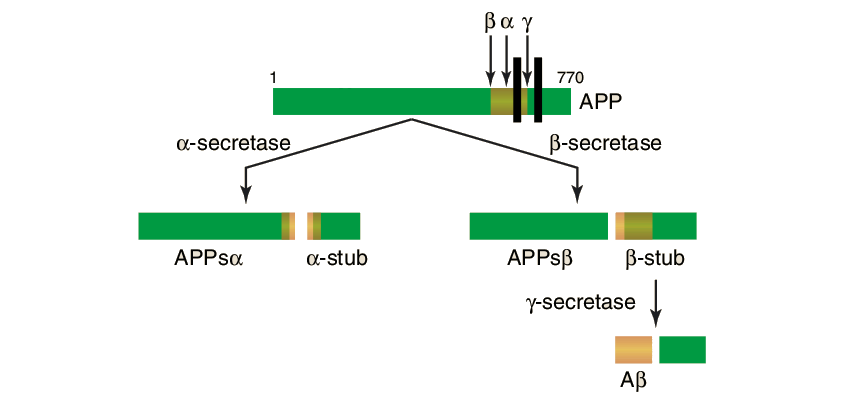
\includegraphics[width=.5\linewidth]{immagini/APP.png}
	\caption{Azione degli enzimi $\alpha$/$\beta$/$\gamma$-secretasi sul substrato APP.}
	\label{fig:app}
\end{figure}

I frammenti prodotti sono di due varietà: gli A$\beta$-40 e i A$\beta$-42, rispettivamente formati da 40 e 42 amminoacidi. La forma A$\beta$-42 tende a formare oligomeri e fibrille più facilmente rispetto all’A$\beta$-40 molto probabilmente vista la minore solubilità data dai due residui idrofobici in più.
La produzione di A$\beta$ in piccole quantità é un processo normale; l'anormalità legata alla comparsa del morbo è da ricercarsi in una disproporzione tra le due specie causata da una scarsa attività di demolizione o eccessiva produzione. \cite{brothers_physiological_2018}

All'aumento della concentrazione di A$\beta$ nel liquido cerebrospinale è associata la tendenza alla formazione di aggregati proteici più grandi ed insolubili detti comunemente "placche" o "fibrille". I fenomeni di aggregazione sono stati osservati anche in presenza di concentrazioni anomale a livello cerebrale di ioni metallici come Zinco, Rame e Ferro.
L'accumulo porta ad alterazione della chimica delle sinapsi, rallentando la trasmissione tra neuroni fino al punto di impedirla, causando così infine la morte della cellula. Inoltre una quantità estremamente alta di specie altamente ossidanti si concentra in questi aggregati di A$\beta$ dando vita a problemi di stress ossidativo.

\section{Strategie d'Intervento}
Visto il complesso sistema che regola la comparsa dei A$\beta$ vien da sè che anche i metodi per cercare di limitarne la presenza o gli effetti sull'organismo saranno altrettanto variegati.
Le metodologie d'intervento studiate nel panorama della ricerca biomedica sono le più disparate. Limitandoci solo a tecniche la cui azione è incentrata direttamente sui A$\beta$ o sui loro effetti in questo elaborato ci soffermeremo sulla modulazione della neurotrasmissione in modo da limitare l'effetto d'inibizione sinaptico, mitigazione degli effetti da stress ossidativo e limitazione dell'aggregazione degli A$\beta$ in oligomeri. \cite{kumar_review_2015}


\section{Resveratrolo}
\label{sec:resv}
Il Resveratrolo è un polifenolo presente in molte piante, in particolare nella buccia e nei semi dell'uva. Alcuni studi hanno evidenziato anche diverse altre funzioni biologiche importanti come antiossidante, antinfiammatorio, fitoestrogeno e cardioprotettore. Anche nel campo delle malattie neurodegenerative il Resveratrolo presenta alcune potenzialità; sono stati osservati effetti di riduzione dell'aggregazione dei A$\beta$, una modulazione della neurotrasmissione mediata da Acetilcolina e riduzione delle specie ossidanti (ROI). \cite{jabir_cholinesterase_2018}

La molecola pur essendo presente in natura in quantità apprezzabili in una grande varietà di piante non è fruibile al punto da coprire la domanda che le applicazioni in campo medico e di ricerca richiedono. Risulta quindi chiara l'importanza di un metodo di sintesi dai bassi costi e facilmente realizzabile.

Uno dei metodi più semplici ed efficaci per sintetizzare la molecola di Resveratrolo può essere realizzato mediante un accoppiamento di Heck-Mizoroki, ovvero attraverso un processo catalitico a base di Palladio.
Nel caso del Resveratrolo la sintesi a partire da reagenti commerciali (rappresentata in Figura \ref{fig:totale_resveratrolo}) è composta di due passaggi sintetici. I reagenti di partenza utilizzati per l'accoppiamento sono lo 1-iodo-3,5-dimetossibenzene ed il 4-metossistirene. Il catalizzatore impiegato è un catalizzatore di palladio nanoparticellare disperso su di un supporto di argilla laponite ottenuto per riduzione di \ce{H2PdCl4} in presenza di polivinilpirrolidone (PVP). \cite{martinez_extremely_2015}
I vantaggi di tale catalizzatore sono l'alta capacità di utilizzo e rigenerazione oltre ad una bassissima quantità di Palladio residuo nei prodotti finali.

In seguito all'accoppiamento, per ottenere la molecola di Resveratrolo si effettua una demetilazione sul prodotto della reazione d'accoppiamento con \ce{BBr3} in diclorometano. \cite{alejandro_v._martinez_expedient_2017}

\begin{figure}[H]
	\centering
	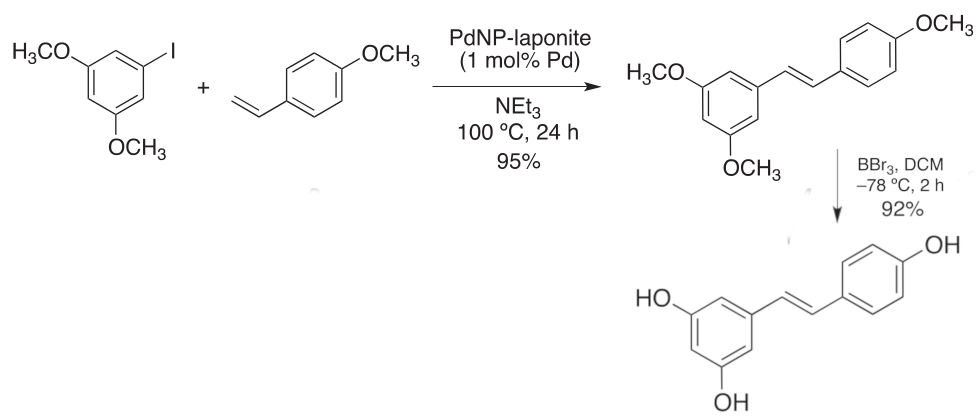
\includegraphics[width=.7\linewidth]{immagini/totale_resveratrolo.png}
	\caption{Reazione di accoppiamento di Heck-Mizoroki seguita dalla deprotezione della funzione metilica per ottenere la maolecola di Resveratrolo.}
	\label{fig:totale_resveratrolo}
\end{figure}

Il Resveratrolo funge da inibitore dell'Acetilcolinesterasi, in particolare l'inibizione è promossa da alcuni suoi tetrameri (Vitisina A e Heyneanol A). L'efficacia e la selettività per i due oligomeri è stata valutata tramite un biotest HPLC restituendo ottimi risultati. In cellule PC12 sono state valutate anche la diminuzione della mortalità cellulare per apoptosi e una diminuzione di specie ROI.

\section{Curcumina}
La Curcumina è la principale componente polifenolica della Curcuma; tale molecola è impiegata nel trattamento di molteplici malattia umane già da migliaia di anni, le prime applicazioni risalgono alla antica medicina cinese.  L'azione della molecola nei confronti dell'AD è attribuibile ad una mitigazione all'aggregazione dei A$\beta$ e all'inibizione dell'enzima AChE. Il principale vantaggio derivante dall'uso della Curcumina come punto di partenza per lo sviluppo di un farmaco per l'AD è la sua innata permeabilità della barriera emato-encefalica. Mi sono soffermato in questa sezione sulla sintesi di composti ottenuti dall'accoppiamento dei farmacofori della Curcumina e del Donepezil, farmaco la cui azione è mirata alla modulazione dell'enzima AChE.

Sono state selezionate due serie di composti da sintetizzare la cui sostanziale differenza risiede nella diversa geometria con cui i due farmacofori sono fusi assieme; gli scheletri molecolari su cui sono state inserite diverse modificazioni sono riportati in Figura \ref{fig:generale_curcdone}.
\begin{figure}[H]
	\centering
	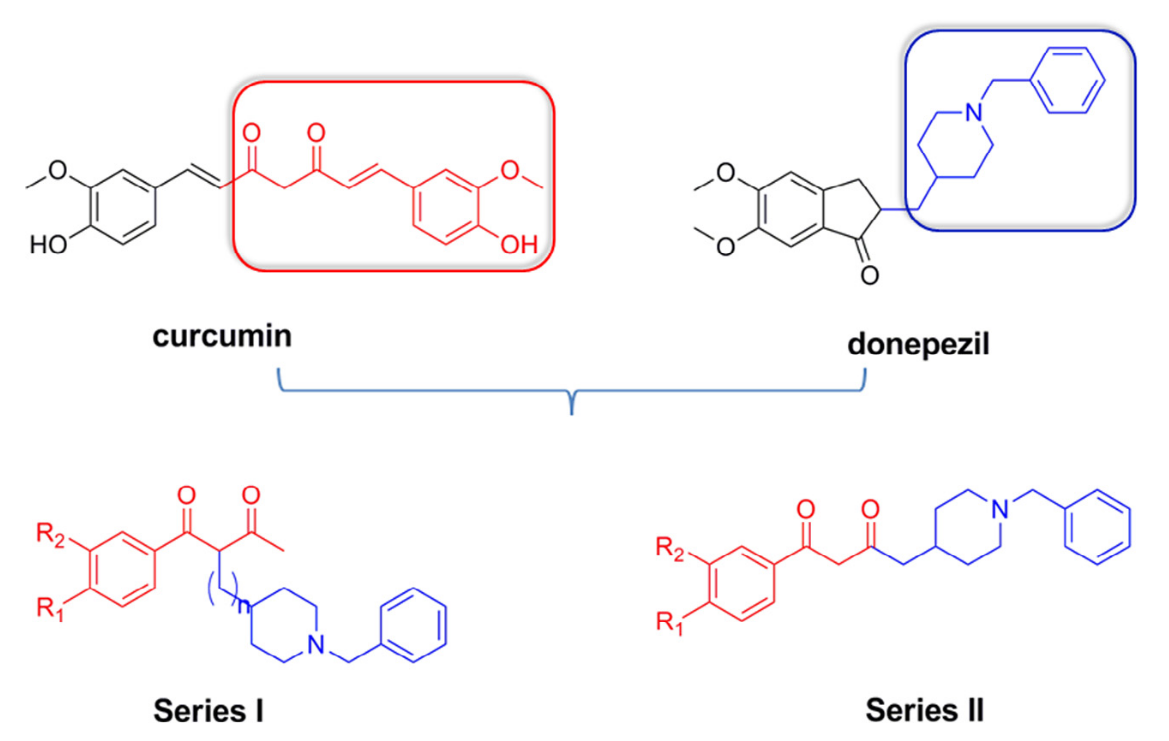
\includegraphics[width=.5\linewidth]{immagini/generale_curcdone.png}
	\caption{Formule di struttura dei composti ottenuti per fusione dei farmacofori appartenenti alla Curcumina (in rosso) e al Donepezil (in blu).}
	\label{fig:generale_curcdone}
\end{figure}

Il processo di sintesi prevede, a partire da reagenti commerciali, la sintesi dei due farmacofori desiderati tra loro accoppiati attraverso reazioni di condensazione. Le molecole sono state differenziate tra loro inserendo in fase di sintesi sostituenti differenti per valutare quali funzionalità possano comportare un miglioramento dell'azione sull'organismo.

Al fine di valutare gli effetti dei prodotti ottenuti sono stati condotti test circa l'attività d'inibizione e la selettività per l'enzima AChE. Inoltre sono stati considerati fattori come la permeabilità della barriera emato-encefalica, diminuzione della concentrazione delle specie ROI e mitigazione dell'aggregazione dei A$\beta$.

I risultati hanno evidenziato una migliore azione nei confronti della malattia per i composti appartenenti alla seconda serie di composti (sempre con riferimento alla Figura \ref{fig:generale_curcdone}), in particolare la presenza sulla molecola di sostituenti idrossilici uniti ad un basso ingombro sterico sono risultati fattori fondamentali per massimizzare l'azione dal punto di vista farmacologico. \cite{jun_yan_design_2017}

\section{Leganti Bipiridinici}
L'ultima classe di composti studiata è quella dei bipiridinici. I composti bipiridinici presentano una buona capacità chelante rispetto agli ioni metallici liberi, la loro azione farmacologica è quindi quella di cercare di limitare l'aggregazione amiloidica diminuendo la quantità di centri di nucleazione per i A$\beta$. Inoltre questa classe di composti presenta una buona permeabilità della barriera emato-encefalica, una buona solubilità in ambiente acquoso e un'alta cinetica di complessazione nei confronti dei metalli; tutti fattori che candidano le bipiridine come ottimi precursori di agenti per la cura dell'AD.

La sintesi si prefigge lo scopo di poter ottenere molecole con le proprietà farmacologiche desiderate inserendo sulle molecole sostituenti che si suppone siano in grado di avere effetto sul substrato voluto.

In questo caso particolare le funzioni inserite sui due anelli piridinici sono state un gruppo metilico per migliorare l'effetto di chelazione metallica e un gruppo dimetilamminico per la sua affinità verso i frammenti A$\beta$. Le stesse funzionalità sono state inserite in posizioni differenti in modo da ottenere prodotti finali tra loro diversi strutturalmente, ciò ha permesso uno studio di quale dei diversi isomeri di struttura potesse migliore da un punto di vista dell'effetto in quanto farmaco.

La sintesi (presentata in maniera schematica in Figura \ref{fig:rea_g}) viene portata a termine per mezzo di un accoppiamento di Stille; la reazione Palladio catalizzata permette la formazione di un nuovo legame carbonio-carbonio tra l'organostannano ottenuto dalla 4-dimetilamminopiridina e l'appropriata piridina bromurata.

\begin{figure}[H]
	\centering
	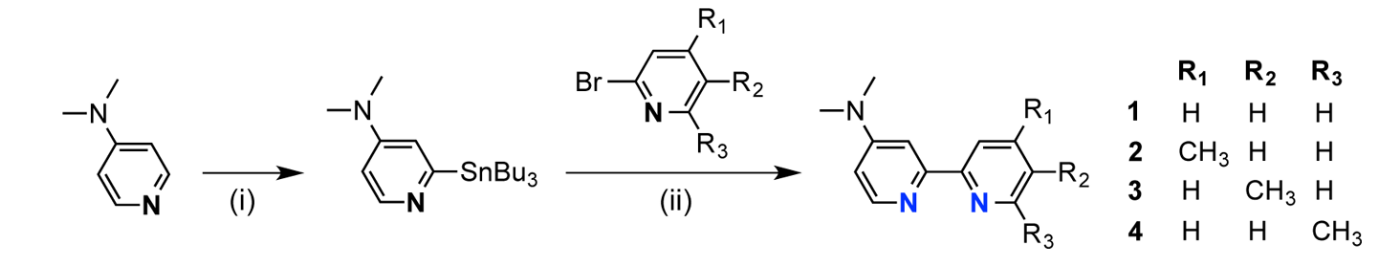
\includegraphics[width=.8\linewidth]{immagini/rea_g.png}
	\caption{Reazione generale per l'ottenimento dei composti d'interesse 1-4. (i) n-BuLi, 2-Dimetilaminoetanolo, Esano, 0 $^\circ$C; \ce{Bu3SnCl}, -78 $^\circ$C; (ii) \ce{PdCl2(PPh3)2}, \ce{LiCl}, \ce{PPh3}, Toluene, 110 $^\circ$C }
	\label{fig:rea_g}
\end{figure}

L'efficacia dei composti sintetizzati è stata valutata mediante test in vitro. In assenza di metalli le bipiridine non hanno mostrato particolari effetti positivi nei confronti della formazione delle placche proteiche; in presenza di ioni metallici l'effetto di chelazione si è dimostrato efficace mitigando in maniera significativa la formazione di cumuli amiloidici. Malgrado la positiva azione nei confronti dei fenomeni di aggregazione e la comprovata capacità di permeazione della barriera emato-encefalica, esperimenti su cellule in vitro hanno evidenziato una discreta citotossicità dei composti comportando una evidente mortalità cellulare per apoptosi. \cite{ji_strategic_2017}

\section{Conclusioni}
In conclusione, la ricerca di una cura al morbo d'Alzheimer è un campo ancora molto aperto; le ipotesi circa le cause che comportano il presentarsi della patologia sono tante e non completamente chiarite. In questo lavoro di tesi mi sono soffermato soltanto su una delle tante sfaccettature del mondo della ricerca in questo campo. I tre casi da me presentati sono un esempio di ciò che la chimica organica può offrire nel tentativo di individuare una possibile cura: usando molecole naturali come base per la sintesi di composti ad esse ispirati in grado di permeare la barriera emato-encefalica e fornire effetti antiossidanti e/o di limitare l'aggregazione proteica come nel caso di Resveratrolo e Curcumina; oppure realizzando tramite un approccio razionale alla sintesi molecole ad hoc in grado di avere gli effetti desiderati sull'organismo come i composti bipiridinici presentati.




\printbibliography

\end{document}
